\documentclass[journal,10pt,romanappendices]{IEEEtai}
\usepackage[utf8]{inputenc}
\usepackage[T1]{fontenc}
\usepackage{amsmath,amssymb,amsthm,mathtools}
\usepackage{booktabs,graphicx,microtype,placeins,array,needspace}
\usepackage[numbers,sort&compress]{natbib}
\usepackage{xurl,hyperref}
\usepackage{xr}
\newcommand{\ArticleTitle}{A Two-Grid Characterization of Euler Sampling Accuracy in Flow Matching}
\hypersetup{pdftitle={A Two-Grid Characterization of Euler Sampling Accuracy in Flow Matching},pdfauthor={Dev D. Goyal},pdflang={en-US},colorlinks=true,linkcolor=blue,citecolor=blue,urlcolor=blue}
\newtheorem{theorem}{Theorem}
\newtheorem{proposition}[theorem]{Proposition}
\newtheorem{lemma}[theorem]{Lemma}
\newtheorem{corollary}[theorem]{Corollary}
\theoremstyle{definition}
\newtheorem{definition}{Definition}
\newcommand{\R}{\mathbb R}
\newcommand{\E}{\mathbb E}
\newcommand{\tr}{\operatorname{tr}}
\newcommand{\Law}{\operatorname{Law}}
\newcommand{\dd}{\,\mathrm d}

\newcommand{\AIcitations}{\citep{openai_chatgpt,openai_codex,anthropic_claude,anthropic_claude_fable}}
\newcommand{\AIassistance}{\footnote{AI assistance for this section is disclosed in the acknowledgment~\AIcitations.}}

\externaldocument{../build/supplement-labels}
\newcommand{\IntroExactFlow}{$1.02$}
\newcommand{\RiskMeshThreshold}{1.3\times10^{-14}}
\newcommand{\RiskStepCount}{7.7\times10^{13}}
\newcommand{\ScalarCfmArgminEight}{0}
\newcommand{\ScalarCfmArgminLast}{3}
\newcommand{\ScalarCfmArgminSixteen}{0}
\newcommand{\ScalarCfmBias}{0.091}
\newcommand{\ScalarCfmBiasMax}{0.195}
\newcommand{\ScalarCfmBiasMin}{0.023}
\newcommand{\ScalarCfmEight}{0.174}
\newcommand{\ScalarCfmFromSixteenIncreaseLarge}{0}
\newcommand{\ScalarCfmFromSixteenIncreaseSixtyFour}{0}
\newcommand{\ScalarCfmFromSixteenWilcoxonLarge}{0.002}
\newcommand{\ScalarCfmFromSixteenWilcoxonSixtyFour}{0.002}
\newcommand{\ScalarCfmIncreaseLarge}{0}
\newcommand{\ScalarCfmIncreaseSixteen}{0}
\newcommand{\ScalarCfmIncreaseSixtyFour}{0}
\newcommand{\ScalarCfmLarge}{0.090}
\newcommand{\ScalarCfmOwnEight}{0.153}
\newcommand{\ScalarCfmOwnLarge}{0.005}
\newcommand{\ScalarCfmPairCoarse}{0.174}
\newcommand{\ScalarCfmPairFine}{0.115}
\newcommand{\ScalarCfmSdMax}{0.063}
\newcommand{\ScalarCfmSixteen}{0.115}
\newcommand{\ScalarCfmSixtyFour}{0.090}
\newcommand{\ScalarCfmWilcoxonLarge}{0.002}
\newcommand{\ScalarCfmWilcoxonSixteen}{0.002}
\newcommand{\ScalarCfmWilcoxonSixtyFour}{0.002}
\newcommand{\ScalarExactBias}{0.000}
\newcommand{\ScalarExactEight}{0.151}
\newcommand{\ScalarExactLarge}{0.005}
\newcommand{\ScalarExactOwnEight}{0.151}
\newcommand{\ScalarExactOwnLarge}{0.005}
\newcommand{\ScalarExactSdMax}{0.000}
\newcommand{\ScalarExactSixteen}{0.077}
\newcommand{\ScalarExactSixtyFour}{0.020}
\newcommand{\ScalarModelCount}{30}
\newcommand{\ScalarOneArgminEight}{6}
\newcommand{\ScalarOneArgminLast}{0}
\newcommand{\ScalarOneArgminSixteen}{4}
\newcommand{\ScalarOneBias}{0.125}
\newcommand{\ScalarOneBiasMax}{0.193}
\newcommand{\ScalarOneBiasMin}{0.084}
\newcommand{\ScalarOneEight}{0.085}
\newcommand{\ScalarOneFromSixteenIncreaseLarge}{10}
\newcommand{\ScalarOneFromSixteenIncreaseSixtyFour}{10}
\newcommand{\ScalarOneFromSixteenWilcoxonLarge}{0.002}
\newcommand{\ScalarOneFromSixteenWilcoxonSixtyFour}{0.002}
\newcommand{\ScalarOneGridFactor}{1.4}
\newcommand{\ScalarOneIncreaseLarge}{10}
\newcommand{\ScalarOneIncreaseSixteen}{6}
\newcommand{\ScalarOneIncreaseSixtyFour}{10}
\newcommand{\ScalarOneLarge}{0.122}
\newcommand{\ScalarOneOwnEight}{0.125}
\newcommand{\ScalarOneOwnLarge}{0.004}
\newcommand{\ScalarOnePairCoarse}{0.085}
\newcommand{\ScalarOnePairFine}{0.084}
\newcommand{\ScalarOneSdMax}{0.041}
\newcommand{\ScalarOneSixteen}{0.084}
\newcommand{\ScalarOneSixtyFour}{0.113}
\newcommand{\ScalarOneWilcoxonLarge}{0.002}
\newcommand{\ScalarOneWilcoxonSixteen}{0.695}
\newcommand{\ScalarOneWilcoxonSixtyFour}{0.002}
\newcommand{\ScalarTwoArgminEight}{0}
\newcommand{\ScalarTwoArgminLast}{0}
\newcommand{\ScalarTwoArgminSixteen}{9}
\newcommand{\ScalarTwoBias}{0.096}
\newcommand{\ScalarTwoBiasMax}{0.127}
\newcommand{\ScalarTwoBiasMin}{0.062}
\newcommand{\ScalarTwoEight}{0.092}
\newcommand{\ScalarTwoFromSixteenIncreaseLarge}{10}
\newcommand{\ScalarTwoFromSixteenIncreaseSixtyFour}{10}
\newcommand{\ScalarTwoFromSixteenWilcoxonLarge}{0.002}
\newcommand{\ScalarTwoFromSixteenWilcoxonSixtyFour}{0.002}
\newcommand{\ScalarTwoIncreaseLarge}{5}
\newcommand{\ScalarTwoIncreaseSixteen}{0}
\newcommand{\ScalarTwoIncreaseSixtyFour}{4}
\newcommand{\ScalarTwoLarge}{0.093}
\newcommand{\ScalarTwoOwnEight}{0.126}
\newcommand{\ScalarTwoOwnLarge}{0.004}
\newcommand{\ScalarTwoPairCoarse}{0.092}
\newcommand{\ScalarTwoPairFine}{0.069}
\newcommand{\ScalarTwoSdMax}{0.026}
\newcommand{\ScalarTwoSixteen}{0.069}
\newcommand{\ScalarTwoSixtyFour}{0.085}
\newcommand{\ScalarTwoWilcoxonLarge}{0.846}
\newcommand{\ScalarTwoWilcoxonSixteen}{0.002}
\newcommand{\ScalarTwoWilcoxonSixtyFour}{0.375}
\newcommand{\VarMediumAllSix}{0.0}
\newcommand{\VarMediumAnySix}{7}
\newcommand{\VarMediumCfmFractionMax}{0}
\newcommand{\VarMediumChangeMean}{-0.015}
\newcommand{\VarMediumChangeSd}{0.005}
\newcommand{\VarMediumFractionMax}{7}
\newcommand{\VarMediumFractionMin}{0}
\newcommand{\VarMediumGridLongFraction}{100}
\newcommand{\VarMediumGridLongMean}{0.014}
\newcommand{\VarMediumLongOneA}{100}
\newcommand{\VarMediumLongOneB}{30}
\newcommand{\VarMediumLongOneC}{77}
\newcommand{\VarMediumLongTwoA}{33}
\newcommand{\VarMediumLongTwoB}{7}
\newcommand{\VarMediumLongTwoC}{20}
\newcommand{\VarMediumSets}{30}
\newcommand{\VarSetCount}{230}
\newcommand{\VarSmallAllSix}{2.5}
\newcommand{\VarSmallAnySix}{43}
\newcommand{\VarSmallCfmFractionMax}{0}
\newcommand{\VarSmallChangeMean}{-0.011}
\newcommand{\VarSmallChangeSd}{0.014}
\newcommand{\VarSmallFractionMax}{38}
\newcommand{\VarSmallFractionMin}{6}
\newcommand{\VarSmallGridLongFraction}{74}
\newcommand{\VarSmallGridLongMean}{0.016}
\newcommand{\VarSmallLongOneA}{74}
\newcommand{\VarSmallLongOneB}{48}
\newcommand{\VarSmallLongOneC}{65}
\newcommand{\VarSmallLongTwoA}{58}
\newcommand{\VarSmallLongTwoB}{29}
\newcommand{\VarSmallLongTwoC}{50}
\newcommand{\VarSmallSets}{200}

\title{\ArticleTitle}
\author{Dev D. Goyal}
\markboth{Two-grid Euler accuracy}{Two-grid Euler accuracy}
\begin{document}
\maketitle
\begin{abstract}

A flow-matching model learns a velocity field that moves noise toward a
data distribution. More solver steps can follow this field more closely
yet produce a worse match to the data. This can happen because numerical
error offsets an error in the field. We ask what accuracy at two step
counts reveals about the field. We run explicit Euler with the same field
from Gaussian noise on a grid of $N$ steps and on the grid that halves
each step. At the shared times, we compare both outputs with the target
distributions using the quadratic Wasserstein distance. Under common
derivative bounds, the sum of these errors can decrease faster than
$1/N$ exactly when a limit of the allowed fields generates the target
path and its acceleration preserves each distribution. Second-order
accuracy is then possible. Otherwise the error sum is at least a
positive constant times $1/N$ on all sufficiently fine grids. For the
path that joins independent noise and data by straight lines, this lower
bound holds in odd dimension for centered targets with positive definite
covariance. For a scalar Gaussian path on uniform grids, the sharp
constant is $(2+\pi)/8$. For each of 20 scalar neural fields fitted at
small step counts, going from 16 to 64 steps reduces the integration
error and increases the error against the target. This difference matters
when a sampler is used at a different step count from the one used in
training.
\end{abstract}

\begin{IEEEImpStatement}

Flow-matching models use numerical steps to generate samples. With
explicit Euler, each step evaluates the learned network once, so changing
the step count changes the cost of sampling. We show why a model that
works well at one step count can give worse samples at another. More
steps bring the solver closer to the exact motion, but a coarse solver
can offset some of the error in the field itself. Our theory gives
conditions under which the output can stay accurate at two step counts.
In the experiments, we also find that a small evaluation set can reverse
the apparent direction of an improvement. When comparing samplers, report
the error against the target and the integration error separately. Give
the step counts, the times used for comparison, and the evaluation set.
\end{IEEEImpStatement}
\begin{IEEEkeywords}
Flow matching, generative models, numerical integration, optimal
transport, ordinary differential equations, sampling efficiency.
\end{IEEEkeywords}

\section{Introduction}
Flow matching trains a neural network to give a \emph{velocity
field}~\citep{lipman2023flow,liu2023flowstraight,albergo2023building}.
The field tells a particle how to move at each time and position. An
ordinary differential equation (ODE) describes this motion, and the
motion carries random noise to a data distribution. Diffusion models
have an equivalent deterministic sampler~\citep{song2021scorebased}, and
large image models use this
method~\citep{esser2024scaling}.\AIassistance

\begin{figure*}[t]
\centering
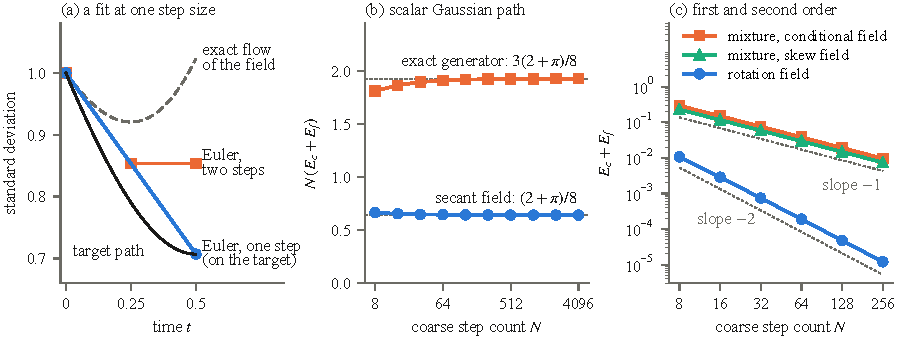
\includegraphics[width=\textwidth]{figures/fig1_rates.pdf}
\caption{Exact population computations. (a) A field that is fitted to
one Euler step of size $1/2$ gives the target standard deviation at time
$1/2$. Two steps of size $1/4$ with the same field do not. (b) For the
scalar Gaussian path of Section~\ref{sec:sharpness}, the scaled two-grid
error $N(E_c+E_f)$ converges to $(2+\pi)/8$ for the secant field and to
three times that value for the exact generator. (c) The two-grid error
decays at first order for two exact generators of a three-dimensional
mixture path, and at second order for a rotation field whose
acceleration preserves each distribution.}
\label{fig:rates}
\end{figure*}

A sampler solves the ODE with a numerical method in a finite number of
steps. Each step uses at least one evaluation of the network, so the
step count sets the cost of each sample. Much work decreases this count
with better solvers~\citep{lu2022dpmsolver,karras2022elucidating,zhang2023fast,shaul2024bespoke},
with straighter
trajectories~\citep{pooladian2023multisample,tong2024improving,lee2023minimizing},
and with models that are trained for few
steps~\citep{salimans2022progressive,song2023consistency,frans2025shortcut,geng2025meanflow}.
Each method tunes a field or a solver for some step counts.

Two different errors occur. The \emph{integration error} is the distance
between the numerical run and the exact motion of the learned field. The
\emph{target error} is the distance between the numerical distribution
and the intended distribution. On fine grids, Euler approaches the exact motion. The target error can
still increase if the coarse run offsets part of the field's error.

Fig.~\ref{fig:rates}(a) gives an example with a one-dimensional Gaussian
(normal) distribution. The standard deviation is $1$ at the start, and
the target standard deviation at time $1/2$ is approximately $0.71$.
Section~\ref{sec:sharpness} gives a field for which one Euler step to
time $1/2$ gives the target distribution exactly. Two steps of length
$1/4$ with the same field give a standard deviation of approximately
$0.85$, and the exact motion of the field gives \IntroExactFlow{}. The
one large step offsets an error of the field. A smaller step removes the
offset.

Prior work explains the forward direction of this effect. Different
velocity fields can generate the same distributions at every
time~\citep{horvat2024gauge}. Take a field that generates the target
path. Only the part of its acceleration that changes the distribution
controls the leading Euler error. A field without that part permits a
higher order~\citep{obzherin2026density,obzherin2026finite}. We ask the converse question for a field that can be biased. If the
same field is accurate with $N$ and $2N$ Euler steps, what does that
accuracy show about the field?

The answer is a property of the continuous motion. In each comparison we
use one field on both grids. Across comparisons, the field can change
with the step count if all fields satisfy the same derivative bounds. Suppose
that the two target errors decay faster than $1/N$. Then a limit of the
allowed fields generates the full target path, and its acceleration
preserves each distribution. If no such limit exists, the sum of the two target
errors has a first-order lower bound. Our contributions are as follows.
\begin{itemize}
\item \emph{Two-grid characterization.} Theorem~\ref{thm:characterization}
gives the equivalence and the uniform lower bound $c/N$. It separates
three regimes of the best two-grid error: a positive limit, first order,
and second order.
\item \emph{Bound at finite step counts.} Theorem~\ref{thm:quantitative-main}
uses the two target errors to bound the part of the acceleration that
changes the distributions of the field. We identify the grid refinements
and the pairs of solvers that permit this inference.
\item \emph{Independent interpolation path.} A common path joins
independent noise and data by straight lines. For this path,
Theorem~\ref{thm:odd-transfer} proves the first-order lower bound in
every odd dimension and for all targets with positive definite
covariance. Theorem~\ref{thm:source-risk}
gives a necessary condition on the regression loss at time zero in every
dimension.
\item \emph{Sharpness.} A scalar Gaussian path has the sharp constant
$(2+\pi)/8$. Examples show that the smoothness assumptions and the use
of intermediate times are necessary.
\item \emph{Experiments.} Exact population computations agree with the
predicted rates. Learned scalar fields show, in the population
Wasserstein distance, how a fit at small step counts trades numerical
error against model bias. A study of \VarSetCount{} evaluation sets measures how sample size
affects a comparison of two step counts.
\end{itemize}



\section{Problem and Regularity Class}
\label{sec:setting}
A probability path $(p_t)_{0\le t\le T}$ gives the target distribution
at each time. We measure the distance between two distributions with the
quadratic Wasserstein distance $W_2$~\citep{villani2009optimal}. Pair
the points of the two distributions and take the root mean squared
distance between paired points. The smallest value over all pairings is
$W_2$. A joint distribution of paired points is a \emph{coupling}. If
numerical and exact particles start from the same point, they give one
coupling, and its error is an upper bound on $W_2$.\AIassistance

Fix a final time $0<T\le1$, a dimension $d\ge1$, and a derivative bound
$K\ge1$. Let $p_t$ be a $W_2$-continuous path of distributions with
finite second moment that starts at the standard Gaussian
$p_0=\gamma_d=\mathcal N(0,I_d)$. We write $\E$ for expectation and
$|x|$ for the Euclidean norm. Let $\mathcal B_K$ be the class of twice
continuously differentiable ($C^2$) velocity fields $u$ on a
neighborhood of $[0,T]\times\R^d$ that satisfy
\begin{equation}
\begin{aligned}
 |u(t,x)|,\ |\partial_tu(t,x)|&\le K(1+|x|),\\
 |\partial_{tt}u(t,x)|&\le K(1+|x|)^2,\\
 \|D_xu\|,\ \|D_x\partial_tu\|,\ \|D_x^2u\|&\le K.
\end{aligned}
\label{eq:budget}
\end{equation}
Here $D_x$ is the derivative in space, $\partial_t$ is the derivative in
time, and $\|\cdot\|$ is the operator norm. The bounds hold at every
point of $[0,T]\times\R^d$. They limit how quickly the velocity can
change in space and in time. They are not bounds on the size of a
network.

A sequence of fields in this class can converge to a field outside the
class. We write $\overline{\mathcal B}_K$ for the closure of
$\mathcal B_K$ in $C^1_{\rm loc}$, in which the fields and their first
derivatives converge uniformly on each compact set. The closure is compact. Each sequence has a subsequence that converges
in this sense. The first derivatives of a limit field are locally
Lipschitz. On each compact set, their change is at most a constant
times the distance between the inputs.

Let $F^u_{s,t}(x)$ be the position at time $t$ of the particle that is
at $x$ at time $s$ and that solves $\dot X_t=u(t,X_t)$. The field has
its own distributions $\rho_t^u=(F^u_{0,t})_\#\gamma_d$, which are the
distributions of $X_t^u=F^u_{0,t}(G)$ for $G\sim\gamma_d$. A fitted
field need not satisfy $\rho_t^u=p_t$. The \emph{model bias} is
$\mathfrak b(u)=\sup_tW_2(\rho_t^u,p_t)$. Let $\Law(X)$ be the
distribution of a random variable $X$. On a grid
$\mathcal T=(0=t_0<\dots<t_N=T)$ with steps $h_k=t_{k+1}-t_k$ and
$H=\max_kh_k$, explicit Euler computes
\[
 \widehat X_{k+1}=\widehat X_k+h_ku(t_k,\widehat X_k),\qquad
 \widehat X_0\sim\gamma_d.
\]
Divide each interval into two equal parts and run Euler again with the
same field and the same initial distribution. Let $\widetilde X_{2k}$ be
the state of this refined run at the coarse time $t_k$. The coarse
error, the refined error, and the \emph{two-grid error} are
\begin{align}
 E_c(u,\mathcal T)&=\max_kW_2(\Law(\widehat X_k),p_{t_k}),\notag\\
 E_f(u,\mathcal T)&=\max_kW_2(\Law(\widetilde X_{2k}),p_{t_k}),\label{eq:errors}\\
 \mathcal J_N(u,\mathcal T)&=E_c+E_f.\notag
\end{align}
We measure both errors at the times of the coarse grid. The two runs use
$N$ and $2N$ evaluations of the field.

An \emph{exact generator} is a field with $\rho_t^u=p_t$ for all $t$.
The \emph{acceleration} of a field is
$a_t(x)=\partial_tu(t,x)+D_xu(t,x)u(t,x)$. It is the rate of change of
the velocity of a moving particle.

\begin{definition}[Order-elevating generator]
A field $u\in\overline{\mathcal B}_K$ is an order-elevating generator of
$p$ if $\rho_t^u=p_t$ for all $t$ and its acceleration satisfies
\begin{equation}\label{eq:AP}
 \int\nabla\phi(x)\cdot a_t(x)\,p_t(\dd x)=0
\end{equation}
for all smooth functions $\phi$ with compact support and all
$t\in[0,T]$.
\end{definition}

To read~\eqref{eq:AP}, hold the time fixed and move the particles for a
short interval in the direction $a_t$. The integral is the rate of
change of the average of the test function $\phi$. If the integral is zero for all tests, every test average has zero
initial rate of change. Under our regularity assumptions, the motion
with time fixed preserves $p_t$. Particles can still move. We then say that the acceleration
\emph{preserves the distribution}. For a smooth density the condition is
$\nabla\cdot(p_ta_t)=0$~\citep{ambrosio2005gradient}.

\section{Two-Grid Characterization}
\label{sec:characterization}
The first result answers the main question. The two target errors can
decay faster than first order exactly when the closure contains an
order-elevating generator. The result is about the best fields that the
common bounds permit, not about each field in the class.\AIassistance

\begin{theorem}[Two-grid characterization]\label{thm:characterization}
For the target path and the class of Section~\ref{sec:setting}, these
statements are equivalent.
\begin{enumerate}
\item There are step counts $N_j\to\infty$, fields
 $u_j\in\mathcal B_K$, and $N_j$-step grids $\mathcal T_j$ with
 $H_j\to0$ such that $\mathcal J_{N_j}(u_j,\mathcal T_j)=o(N_j^{-1})$.
\item The closure $\overline{\mathcal B}_K$ contains an order-elevating
 generator of $p$.
\item On the uniform grids $t_k=kT/N$, there are fields
 $u_N\in\mathcal B_K$ with $\mathcal J_N(u_N,\mathcal T_N)=O(N^{-2})$.
\end{enumerate}
If the closure contains no order-elevating generator, there are
constants $c,H_0>0$ such that, for every $u\in\mathcal B_K$ and every
deterministic $N$-step grid with $H\le H_0$,
\begin{equation}\label{eq:general-uniform-barrier}
 E_c(u,\mathcal T)+E_f(u,\mathcal T)\ge c/N.
\end{equation}
The field and the grid can change with $N$. Each pair of a coarse run
and a refined run must use one field.
\end{theorem}

The notation $o(N^{-1})$ means that $N$ times the error tends to zero,
and $O(N^{-2})$ means that the error is at most a constant times
$N^{-2}$ for large $N$. The theorem is a statement about the limit
$N\to\infty$. It does not give an error rate from one experiment. The
maximum of the two errors can replace their sum. The constant in the
lower bound then changes by a factor of at most two. The implication
from statement~2 to statement~3 is the direction of the prior
results~\citep[Theorem~2]{obzherin2026density}, \citep[Corollary~8]{obzherin2026finite},
here for limit fields in $\R^d$. The other implications and the lower
bound are new.

\subsection{Proof Idea: Subtract the Two Runs}
Euler uses the velocity at the start of each step. It therefore omits
the displacement $h^2a_t/2$ that the acceleration causes. To see the
effect on a distribution, compare the averages of one scalar test in the
two runs. Let $\phi_t=\phi\circ F^u_{t,0}$ carry a test $\phi$ backward
along the flow of the field, so that its value is constant along each
exact trajectory. Let $I_u(t)=\E[\nabla\phi_t(X_t^u)\cdot a_t(X_t^u)]$
measure how the acceleration changes this average. Each Euler step
changes the average by $-h_k^2I_u(t_k)/2$ to leading order, and these
changes add~\citep{talay1990expansion}:
\[
 \E\phi_{t_j}(\widehat X_j)-\E\phi(G)=-\tfrac12\sum_{k<j}h_k^2I_u(t_k)
 +O\Big(H\sum_{k<j}h_k^2\Big).
\]
The constants are the same for all fields in $\mathcal B_K$ and all
tests with common derivative bounds. In the refined run each step is
divided in two, so the two squared half steps sum to half the squared
coarse step. Subtract the refined expansion from the coarse expansion,
as in step doubling for the estimation of ODE
errors~\citep{richardson1911approximate,hairer1993solving}:
\begin{equation}\label{eq:contrast-main}
 Z_j-Z_i=-\tfrac14\sum_{k=i}^{j-1}h_k^2I_u(t_k)
 +O\Big(H\sum_{k=i}^{j-1}h_k^2\Big).
\end{equation}
Here $Z_k$ is the difference of the two numerical averages at $t_k$.
Both runs have the same exact-flow average, so the unknown model bias
cancels. The target distribution is a common reference for the two runs,
and the triangle inequality gives $|Z_k|\le C(E_c+E_f)$. We do not need
the distance between $\rho_t^u$ and $p_t$.

Suppose that the two-grid error is $o(N^{-1})$ and $H\to0$. Compactness
gives a subsequence of fields with a limit. The integration error of
Euler is $O(H)$ uniformly in the class, so the model bias of these
fields tends to zero, and the limit generates the target path exactly.
Suppose that~\eqref{eq:AP} fails for the limit at some time and for some
test. The flow maps are invertible, so this test is $\phi_t$ for a
suitable $\phi$, and $I_u$ is not zero at that time. Then $I_u$ keeps
one sign on a time interval, also for the fields near the limit. On a fine grid, the first and last nodes in
that interval are separated by at least some $\ell>0$. The squared
steps between them then sum to at least $\ell^2/N$. Equation~\eqref{eq:contrast-main}
then gives a difference of order $1/N$, which contradicts the assumed
accuracy. Thus~\eqref{eq:AP} holds.

Conversely, suppose that an exact generator
satisfies~\eqref{eq:AP}. Move the particles along the acceleration
field for an auxiliary time $h^2/2$ while the physical time is fixed.
This motion changes the pairing of start points but not their
distribution. The new pairing supplies the displacement that Euler
omits, and the one-step $W_2$ error becomes $O(h^3)$. Stability of the
Euler map gives a total error $O(H^2)$. If the generator is only a limit
field, smooth fields in the class approximate both runs. Supplementary
Sections~\ref{app:uniform}--\ref{app:characterization} give the uniform
bounds and the full proof.

\subsection{Three Regimes of the Best Two-Grid Error}
On uniform grids let $q_N=\inf_{u\in\mathcal B_K}\mathcal J_N(u)$ and
$\mathfrak b_*=\min_{u\in\overline{\mathcal B}_K}\mathfrak b(u)$. Three
cases occur, and they depend on what the closure contains:
\begin{equation}\label{eq:regimes}
\begin{array}{@{}ll@{}}
\text{no exact generator:} & q_N\to2\mathfrak b_*>0,\\
\text{exact, not order-elevating:} & q_N=\Theta(N^{-1}),\\
\text{an order-elevating generator:} & q_N=O(N^{-2}).
\end{array}
\end{equation}
Here $\Theta(N^{-1})$ means upper and lower bounds of that order. The three cases separate model bias from numerical error, and they
describe the best fields of the class. The last case includes exact
Euler sampling. For one fixed field, both target errors approach its
model bias as the step count increases.

\section{A Bound at Finite Step Counts}
\label{sec:observable}
Theorem~\ref{thm:characterization} is a limit statement. Two runs at
finite step counts answer a related question, also when the field is
biased. How much can the acceleration change the distributions of the
field?\AIassistance

In a test average, the field is paired with a gradient. Let $L^2(\rho)$
be the space of fields with finite mean squared norm under $\rho$. Let
$\Pi_\rho$ retain the part of a field detected by gradient tests. It is
the orthogonal projection in $L^2(\rho)$ onto the closure of the gradients
of smooth functions with compact
support~\citep{ambrosio2005gradient}. The
\emph{projected-acceleration residual} of a field is
\[
 \varepsilon_t(u)=\|\Pi_{\rho_t^u}a_t\|_{L^2(\rho_t^u)}.
\]
A zero residual means that the acceleration preserves $\rho_t^u$. The
agreement of $\rho_t^u$ with $p_t$ is a separate requirement.

The bound permits general refinements. Divide the coarse interval $k$
into parts with fractions $\theta_{kr}>0$, $\sum_r\theta_{kr}=1$, and
let
\begin{equation}\label{eq:beta-main}
 \beta_k=1-\sum_r\theta_{kr}^2\ge\beta_0>0.
\end{equation}
The number $\beta_k$ is the fraction by which the sum of squared steps
decreases in interval $k$. A refinement is \emph{balanced} if a fixed
$\beta_0>0$ is a lower bound for all $\beta_k$. Division into $m$ equal
parts has $\beta_0=1-1/m$, and bisection has $\beta_0=1/2$. Let $E_r$ be
the target error of the refined run at the coarse nodes, and let
$E=E_c+E_r$. For bisection, $E_r=E_f$.

\begin{theorem}[Finite-step bound on the residual]\label{thm:quantitative-main}
Let $u\in\overline{\mathcal B}_K$, and let the refinement
satisfy~\eqref{eq:beta-main}. Let $\eta=1/3$ for arbitrary grids and
$\eta=1/2$ for uniform grids. For every integer $q\ge0$,
\begin{equation}\label{eq:quantitative-main}
\begin{split}
 \sup_t\varepsilon_t(u)^2\le e^{2KT}\Bigg\{&\sum_{1\le|\alpha|\le q+1}
 \big[L_\alpha H+\Lambda_\alpha(NE)^{\eta}\big]^2\\
 &+\frac{V}{q+1}\Bigg\}.
\end{split}
\end{equation}
The sum is over multi-indices $\alpha=(\alpha_1,\dots,\alpha_d)$ of
total degree $|\alpha|=\sum_i\alpha_i$. The constants $L_\alpha$, $\Lambda_\alpha$, and $V$ are explicit
functions of $K$, $d$, $T$, $\beta_0$, and $\alpha$. Supplementary
Section~\ref{app:observable} gives them, with $V=dM_2V_1^2$ in its
notation. The bound
does not assume that $u$ generates the target path.
\end{theorem}

The bound has two parts. The sum controls finitely many coefficients of
the acceleration in a basis of Gaussian (Hermite)
polynomials~\citep{bogachev1998gaussian}. Each coefficient is a test
average. A large average keeps its sign on a time interval. The
subtraction in~\eqref{eq:contrast-main} then gives a lower bound on the
two target errors. The term $V/(q+1)$ controls the
coefficients of higher degree, which the tests do not measure. It uses a
bound on the derivative of the acceleration in the coordinates of the
Gaussian start. Obzherin and Khrulkov~\citep[Proposition~10]{obzherin2026finite}
separate measured coefficients from an orthogonal remainder. Here the
two runs bound the measured coefficients, and regularity bounds the
remainder.

The bound has this use in the limit. First choose $q$ large to make the
last term small. Then make $H$ and $NE$ small. The full residual then
tends to zero uniformly in time. The constants increase quickly with the
degree, the dimension, and $K$, so the bound is too large for numerical
use in high dimension. A linear bound from tests with bounded
derivatives would be stronger, but it is false. For
$u_n(t,x)=t\sin(nx)/n^2$, which is in $\mathcal B_1$, the residual at
time zero is asymptotic to $1/(\sqrt2n^2)$, while all such test averages
are $O(n^{-3})$.

\subsection{Informative Refinements and Solver Pairs}
A refinement must change the step sizes by a sufficient amount.
Theorem~\ref{thm:characterization} and its lower bound hold for each
balanced refinement, with $\beta_0>0$ common to all comparisons. A
larger step count alone is not sufficient. For example, divide
each step $h=1/N$ into $h/N$ and $h(1-1/N)$. Then $\beta_k=O(1/N)$,
and both target errors can be $O(N^{-2})$ on a path that has no
order-elevating generator. The step counts $N$ and $N+1$ can be equally uninformative.

The same method compares two solvers on one grid. Consider a fixed explicit Runge--Kutta method. Its weights $\mathsf b$
sum to one and each stage time in $c$ equals the sum of its row of stage
coefficients and lies in $[0,1]$. The method has the coefficient $\kappa=1/2-\mathsf b^\top c$ in its leading
particle error $-\kappa h^2a$~\citep{hairer1993solving}.
If two methods have different values of $\kappa$, their leading errors
remain after subtraction, and the characterization holds with their two
target errors (Supplementary Section~\ref{app:scheme-extension}). Euler
and Heun are one such pair. Two second-order methods both have
$\kappa=0$, so they are not such a pair.

\section{The Independent Interpolation Path}
\label{sec:odd}
We now apply the characterization to a common path. Draw noise and a
data point independently, and interpolate between them:
\begin{equation}\label{eq:independent}
 p_t=\Law((1-t)G+tY),\qquad G\sim\gamma_d,\quad G\perp Y.
\end{equation}
Here $G\perp Y$ means that $G$ and $Y$ are independent. The target $Y$
has mean zero, a finite second moment, and a positive definite
covariance $S$. Restrict the path to an interval
$[0,T]$.\AIassistance

\begin{theorem}[Odd-dimensional obstruction]\label{thm:odd-transfer}
For odd $d$, the path~\eqref{eq:independent} has no order-elevating
generator in $\overline{\mathcal B}_K$. Thus there are constants
$c,H_0>0$ such that~\eqref{eq:general-uniform-barrier} holds for every
field in $\mathcal B_K$ and every $N$-step grid with $H\le H_0$. The
fields need not generate the path.
\end{theorem}

The theorem is not limited to linear fields, Gaussian targets, radial
targets, or one fixed field. For isotropic Gaussian paths and linear
fields, the effect of the parity of the dimension is
known~\citep[Theorem~12]{obzherin2026density}.
Theorem~\ref{thm:odd-transfer} extends it to nonlinear fields and to
targets that are not Gaussian.

\subsection{Why the Start of the Path Decides}
At time zero a particle at $x$ is paired with independent data of mean
zero, so its average interpolation velocity is $-x$. For an exact limit
generator, let $r(x)=u(0,x)+x$ be the difference from this velocity. The
first time derivative of the path gives $\nabla\cdot(\gamma_dr)=0$, so
$r$ does not change the Gaussian start. The second time derivative gives
a second condition. For each unit vector $e$ and each smooth compactly supported scalar
test $\psi$,
\begin{equation}\label{eq:twojet-main}
\begin{split}
 \E[\psi'(e\cdot G)\,e\cdot a_0(G)]
 =\int\psi''(y)\{e^\top Se-Q_e(y)\}\varphi(y)\,\dd y.
\end{split}
\end{equation}
Here $\varphi$ is the standard one-dimensional Gaussian density, and
$Q_e(y)=\E[(e\cdot r(G))^2\mid e\cdot G=y]$ is the mean squared
correction in the direction $e$. If the acceleration preserves the
distribution, the left side is zero for all $\psi$. We therefore look
for an interval of $y$ in which $Q_e(y)$ is smaller than the target
variance $e^\top Se$.

For odd $d\ge3$, a sphere in $\R^d$ has even dimension. The hairy-ball
theorem says that a continuous field tangent to such a sphere is zero at
some point~\citep{hatcher2002algebraic}. Thus the tangential part of $r$
is zero at some point $Re$ of each sphere of radius $R$. Near this
point, the condition $\nabla\cdot(\gamma_dr)=0$ and the Lipschitz
constant ${\rm Lip}(r)$ give $Q_e(y)=O({\rm Lip}(r)^2/R^2)$, while
$e^\top Se\ge\lambda_{\min}(S)>0$. For large $R$, a convex test with
$\psi''$ supported in $[R,R+1]$ makes the right side
of~\eqref{eq:twojet-main} positive. This test has no compact support,
and a cutoff argument extends~\eqref{eq:AP} to it. The positive value
therefore contradicts~\eqref{eq:AP}.
The case $d=1$ is direct. Supplementary Section~\ref{app:source} gives
the proof. The same topological fact gives a related one-step result
in~\citep[Theorem~34]{obzherin2026finite}.

\subsection{Exact Generators Exist, and Even Dimension Is Different}
The obstruction can hold even when an exact generator exists. For
$Y=\mu\xi e_1+\sigma Z$, with an equally likely sign $\xi\in\{-1,1\}$ and an independent
standard Gaussian $Z$, the conditional velocity is a linear field plus a term
$c(t)\tanh(b(t)x_1)e_1$. It generates the path and it
satisfies~\eqref{eq:budget} for a finite $K$.

Odd dimension is necessary. For even $d$ and
$Y\sim\mathcal N(0,\sigma^2I)$, take a matrix $J$ with $J^\top=-J$ and
$J^2=-I$, and let $X_t=((1-t)I+\sigma tJ)G$. This process has the
distributions of~\eqref{eq:independent}, its trajectories are straight
lines, and Euler is exact on every grid. Its field is the skew field
of~\citep[Theorem~12]{obzherin2026density} for this path. The process
uses a different coupling of noise and data but the same path of
distributions.

The obstruction also holds for a class of starts that are not Gaussian.
Supplementary Theorem~\ref{thm:radial-proof} proves it in odd dimension for radial
start densities
$q_W(x)\propto\exp\{-|x|^2/2-W(|x|^2)\}$ with $W\in C^2([0,\infty))$, $W(0)=0$, and $W'\ge0$.
Theorem~\ref{thm:characterization} extends to positive continuous start
densities with a finite fourth moment. The Hermite bound of
Theorem~\ref{thm:quantitative-main} needs the Gaussian start.

\section{A Condition on the Initial Regression Loss}
\label{sec:risk}
Theorem~\ref{thm:odd-transfer} uses only the target. In every dimension,
the regression loss at time zero gives a second test for faster than
first-order accuracy. On the path~\eqref{eq:independent}, flow matching
predicts the displacement $Y-G$. Given $G=x$, the best prediction is
$-x$ because $Y$ has mean zero. Let $\nu=\tr S=\E|Y|^2$. The initial
loss and its excess over the minimum are\AIassistance
\begin{align}
 \mathcal L_0(u)&=\E|u(0,G)-(Y-G)|^2=\nu+\Delta_0(u),\label{eq:loss}\\
 \Delta_0(u)&=\E|u(0,G)+G|^2.\notag
\end{align}
For an exact generator whose acceleration preserves each distribution,
$\Delta_0=\nu$, so the initial loss is twice its minimum. This follows
from the moment bound of~\citep[Proposition~30]{obzherin2026finite} and
the decomposition of the loss~\citep{mei2026ambiguity}. The next result
does not assume exact generation. It uses only the errors of the two
Euler runs.

\begin{theorem}[Initial-loss inequality]\label{thm:source-risk}
For the path~\eqref{eq:independent} in any dimension, where $S$ can be
singular, every $u\in\mathcal B_K$ and every deterministic
$N$-step grid satisfy
\begin{equation}\label{eq:risk-main}
\begin{split}
 |\Delta_0(u)-\nu|\le{}&\omega_K(E_c+C_{\rm path}H)+C_HH\\
 &+\{64D_qN(E_c+E_f)/c_\ell^2\}^{1/3}.
\end{split}
\end{equation}
On the uniform grid $h=T/N$, the last term can be replaced by
\begin{equation}\label{eq:risk-uniform}
 \{32D_qN(E_c+E_f)/(Tc_\ell)\}^{1/2}.
\end{equation}
The constants $C_{\rm path}$, $C_H$, $D_q$, $c_\ell$ and the function
$\omega_K$ are explicit in $K,d,T,\nu$ (Supplementary
Section~\ref{app:risk}). The function $\omega_K$ is nondecreasing, with
$\omega_K(0)=0$ and $\omega_K(b)=O(b^{1/3})$ as $b\to0$. Thus, for fields $u_N\in\mathcal B_K$ on $N$-step grids with
$H_N\to0$, the accuracy $E_c+E_f=o(N^{-1})$ implies
\begin{equation}\label{eq:loss-limit}
 \Delta_0(u_N)\to\nu,\qquad\mathcal L_0(u_N)\to2\nu.
\end{equation}
A fixed gap $|\Delta_0-\nu|\ge g>0$ gives explicit constants
$c_g,H_g>0$ such that $E_c+E_f\ge c_g/N$ on every grid with $H\le H_g$.
\end{theorem}

The proof measures the acceleration at time zero with the
quadratic test $|x|^2/2$ and uses the subtraction of the two runs. It
estimates the first two time derivatives of the second-moment bias by
finite differences. The function $\omega_K$ is the result of the best
choice of the difference interval.

Three limits of this result are important. First, the condition is on the
full expected loss at time zero. An average of the training loss over
sampled times does not establish it. Second, the condition is only
necessary: a three-dimensional skew field has $\Delta_0=\nu$ and an
acceleration that does not preserve the distribution (Supplementary
Section~\ref{app:controls}). A larger regression loss is not a general
method to improve a sampler. Third, the constants are conservative. For
$d=T=K=1$ and $\nu=g=1$, the explicit threshold $H_g$ is approximately
$\RiskMeshThreshold$, which needs approximately $\RiskStepCount$ uniform
steps.

\section{Sharpness}
\label{sec:sharpness}
This section gives the example of Fig.~\ref{fig:rates}(a) in general
form. A field can be exact at one step count and lose this accuracy
after refinement. Let $p_t=\mathcal N(0,g(t)^2I_d)$ with
$g(t)=\sqrt{(1-t)^2+\sigma^2t^2}$ and $\sigma>0$. For the uniform step
$h=1/N$, the \emph{secant field} is\AIassistance
\begin{equation}\label{eq:secant}
 u_h(t,x)=\frac{g(t+h)-g(t)}{h\,g(t)}x.
\end{equation}
Its coefficient uses the change of the target scale over one full step.
On its own grid, each Euler step multiplies each particle by
$g(t+h)/g(t)$. Euler therefore gives each target distribution at the
nodes exactly, in every dimension. These fields have common derivative
bounds. The exact flow of $u_h$ has a bias $\Theta(h)$. If the
\emph{same} field is run with the step $h/2$, the scale of the refined
run is
\begin{equation}\label{eq:sharp-transfer}
 \widehat g_{h/2;u_h}(t)=g(t)\exp\Big\{\frac h4\int_0^t
 \frac{g''(s)}{g(s)}\,\dd s+O(h^2)\Big\}.
\end{equation}
Because $g''/g>0$, we get $E_c=0$ and $E_f=\Theta(h)$. In odd dimension
the sum has the order of the lower bound in
Theorem~\ref{thm:odd-transfer}. Mix the exact coefficient and the
secant coefficient with a weight $\theta$:
$(1-\theta)g'/g+\theta[g(t+h)-g(t)]/[hg(t)]$. The leading coarse and
refined error coefficients are then proportional to $|\theta-1|$ and
$|\theta-1/2|$. Their sum is constant for $1/2\le\theta\le1$. The order
does not change.

\subsection{The Smallest Leading Error in One Dimension}
Let $d=T=1$ and $\sigma=1$. Use uniform grids of $N$ steps and
divide each step into $m$ equal parts. Let $q_N^{(m)}$ be the infimum
of $E_c+E_r$ over all fields in $\mathcal B_K$, not only linear
fields. The
exact generator has the coefficient $c(t)=g'(t)/g(t)$. If $K$ is larger
than this coefficient and its first two derivatives, then
\begin{equation}\label{eq:sharp-main}
 \lim_{N\to\infty}Nq_N^{(m)}=\tfrac12(1-1/m)(1+\pi/2).
\end{equation}
For bisection the constant is $(2+\pi)/8$. The secant field attains it in the limit.
The proof has three steps. In one dimension the exact generator of this
path is unique. For small steps the Euler maps are increasing, so the
pairing of equal quantiles attains $W_2$. An expansion of the particle
error that is uniform over the class then gives the lower bound
(Supplementary Theorem~\ref{thm:sharp-minimax-proof}).

\subsection{Smoothness in Time and Intermediate Times Are Necessary}
A field that oscillates in time can be exact on a grid and on its
bisection at each coarse node. Its first derivatives are bounded, but
its second time derivative increases like $N$. The bound on
$\partial_{tt}u$ in~\eqref{eq:budget} is therefore necessary
(Supplementary Section~\ref{app:scheme-extension}).

An error at the final time alone does not give the lower bound. The
field $u(t,x)=-5t^2x$ on $[0,1]$ generates a Gaussian path. Euler has a
second-order error at the final time for each fixed refinement factor.
Its error over the full path is first order. Acceleration effects of
opposite sign cancel at the final time (Supplementary
Section~\ref{app:observable-geometry}).

\section{Numerical Experiments}
\label{sec:experiments-new}
We first compute the errors for fields with known distribution paths.
Then we measure what happens when networks are trained for a small
number of steps. In one dimension we estimate population errors by
numerical integration. In two dimensions we examine how much the
comparison changes with the evaluation samples.
Supplementary Sections~\ref{app:experiments}--\ref{app:set-variability}
give all settings.\AIassistance

\begin{figure*}[t]
\centering
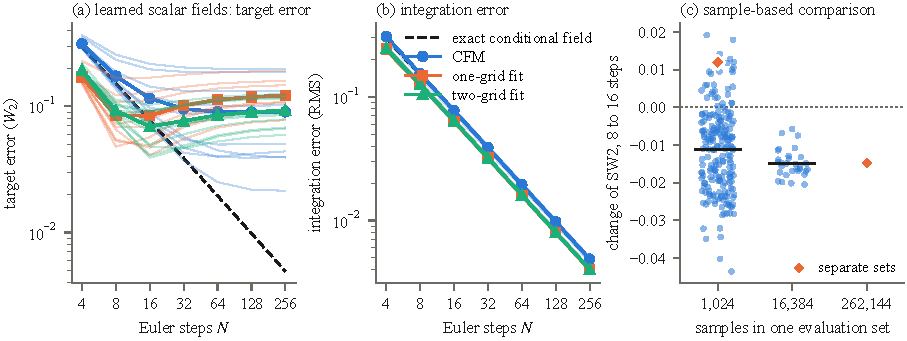
\includegraphics[width=\textwidth]{figures/fig2_learned.pdf}
\caption{Learned fields. (a) Target error of learned scalar fields in
the population $W_2$ distance. Thin lines are the ten seeds of each
objective, and lines with markers are their means. Fields that are
fitted at 8 steps, or at 8 and 16 steps, have their smallest target
error near those step counts. (b) The integration error of the same
fields decreases at first order for all objectives. The legend is for
panels (a) and (b). (c) Change of the
empirical sliced Wasserstein distance (SW2) from 8 to 16 steps,
averaged over six fitted two-dimensional fields. Positive values show
increases. Each dot is one evaluation set. The lines give the means
for each set size, and the diamonds give the values for the separate
sets of 1,024 and 262,144 samples.}
\label{fig:learned}
\end{figure*}

\subsection{Exact Population Computations}
\label{sec:population-example}
Fig.~\ref{fig:rates}(b) shows the scalar Gaussian path of
Section~\ref{sec:sharpness}. For the secant field, $N(E_c+E_f)$ is
$0.666$ at $N=8$ and $0.6428$ at $N=4096$. The limit
in~\eqref{eq:sharp-main} is $(2+\pi)/8\approx0.6427$. The exact
generator has the limit $3(2+\pi)/8$.

Fig.~\ref{fig:rates}(c) shows the two other regimes. For first order,
take the path~\eqref{eq:independent} in dimension three. The first
target coordinate is an equal mixture of Gaussians with means $\pm1.5$
and standard deviation $0.5$. The other two coordinates are centered
Gaussians with the same standard deviation. We compare two exact
generators. The first is the conditional field. The second uses the
skew field of Section~\ref{sec:odd} in the Gaussian plane, which makes
Euler exact in that plane. Theorem~\ref{thm:odd-transfer} gives a lower
bound $c/N$ for both. With the conditional field, $E_c+E_f$ decreases
from $0.292$ at $N=8$ to $0.0096$ at $N=256$. With the skew field, it
decreases from $0.228$ to $0.0074$. The observed orders between $N=128$
and $N=256$ are $0.997$ and $0.998$. The skew field removes the error in
the plane, and the error in the mixture coordinate stays at first order.

For second order, take $d=2$ and the rotation field
$u(t,x)=\tanh(t)x+Jx$, where $J$ is the rotation by a quarter turn. It
generates $p_t=\mathcal N(0,\cosh^2(t)I)$. Its acceleration $2\tanh(t)Jx$ moves particles around circles.
Rotation leaves the Gaussian unchanged, so the acceleration preserves
each $p_t$. Theorem~\ref{thm:characterization} predicts second order.
The scaled error $N^2(E_c+E_f)$ is $0.68$ at $N=8$ and $0.79$ at $N=256$.

\subsection{Learned Scalar Fields With Population Errors}
\label{sec:scalar-learned}
In one dimension, $W_2$ pairs points with the same cumulative
probability. For example, it pairs the two medians. We estimate
population errors by quadrature, which approximates an integral with
a weighted sum. The target is the mixture
coordinate above with the path~\eqref{eq:independent}, so
Theorem~\ref{thm:odd-transfer} applies with $d=1$.

We train networks with two hidden layers of 48 tanh units on three
objectives, with ten random seeds per objective. \emph{CFM} uses the conditional flow
matching loss~\citep{lipman2023flow}. The \emph{one-grid fit} adds a
loss for agreement with the target path in a run of eight Euler steps.
The loss uses the times $1/4$, $1/2$, $3/4$, and $1$. The \emph{two-grid fit} adds
this loss for runs of eight and of sixteen steps. The added loss is the
squared $W_2$ distance between sorted batches. The step size is not an
input of the networks. Training uses
Adam~\citep{kingma2015adam}, and all settings were fixed before the
evaluation.

We report three quantities. The \emph{target error} at $N$ steps is the
largest $W_2$ distance to the target path at the four times. The
\emph{integration error} is the largest root mean squared (RMS) distance
to the exact flow of the field from the same start points. The
\emph{model bias} is estimated as the largest $W_2$ distance between
a reference solution of the flow and the target at 64 times. The errors $E_c$ and $E_f$
of~\eqref{eq:errors} use all nodes of the coarse grid. Supplementary
Table~\ref{tab:scalar-models} gives them for $N=8$.

\begin{table}[t]
\caption{Learned scalar fields: means over ten seeds of population
errors at $N$ Euler steps. The exact field is the conditional velocity,
without training. Supplementary Table~\ref{tab:scalar-models} gives each
field.}
\label{tab:scalar}
\centering
\footnotesize
\begin{tabular}{@{}l@{\hspace{5pt}}c@{\hspace{5pt}}c@{\hspace{5pt}}c@{\hspace{5pt}}c@{\hspace{7pt}}c@{\hspace{7pt}}c@{\hspace{5pt}}c@{}}
\toprule
 & \multicolumn{4}{c}{Target error} & Model & \multicolumn{2}{c@{}}{Integration error}\\
\cmidrule(lr){2-5}\cmidrule(l){7-8}
Field & $N{=}8$ & $16$ & $64$ & $256$ & bias & $N{=}8$ & $256$\\
\midrule
Exact field & 0.151 & 0.077 & 0.020 & 0.005 & 0.000 & 0.151 & 0.005\\
CFM & 0.174 & 0.115 & 0.090 & 0.090 & 0.091 & 0.153 & 0.005\\
One-grid fit & 0.085 & 0.084 & 0.113 & 0.122 & 0.125 & 0.125 & 0.004\\
Two-grid fit & 0.092 & 0.069 & 0.085 & 0.093 & 0.096 & 0.126 & 0.004\\
\bottomrule
\end{tabular}

\end{table}

Table~\ref{tab:scalar} and Fig.~\ref{fig:learned}(a,b) give the results.
The integration error decreases at about first order for all objectives. The
target error does not. For the CFM fields, it decreases from
\ScalarCfmEight{} at 8 steps to \ScalarCfmLarge{} at 256 steps. Their
mean model bias is \ScalarCfmBias{}, with values between
\ScalarCfmBiasMin{} and \ScalarCfmBiasMax{} for the ten seeds. The one-grid fit decreases the mean target error
at 8 steps to \ScalarOneEight{}. For these fields the target error is
larger at 64 steps and at 256 steps than at 8 steps, for all ten seeds.
The exact two-sided Wilcoxon signed-rank test gives
$p=\ScalarOneWilcoxonSixtyFour$ for each of the two comparisons. The change from 8
to 16 steps has no consistent direction: the target error increases for
\ScalarOneIncreaseSixteen{} of the ten seeds ($p=\ScalarOneWilcoxonSixteen$).
Between 8 and 256 steps the mean target error increases by a factor of
\ScalarOneGridFactor{}, while the mean integration error decreases from
\ScalarOneOwnEight{} to \ScalarOneOwnLarge{}. For the two-grid fields,
the target error is smallest at 16 steps for \ScalarTwoArgminSixteen{}
of the ten seeds. For all 20 fitted fields, the target error is larger
at 64 steps and at 256 steps than at 16 steps. The test gives
$p=\ScalarTwoFromSixteenWilcoxonSixtyFour$ for each objective and each
comparison. For all ten CFM fields, the target error is smaller at 64
and at 256 steps than at 16 steps.

For a fixed field, the target error at the four evaluation times
approaches the bias of the exact flow at those times. A coarse run can
offset part of this bias. In the fitted fields, finer runs approach
the exact flow as their error against the target increases. These
comparisons hold the field fixed. Theorem~\ref{thm:characterization}
instead concerns the best error over a class of fields.

\subsection{Sample-Based Comparisons in Two and Eight Dimensions}
\label{sec:sample-based}
In higher dimension, the target error is estimated from samples. We
test how reliable a comparison of two step counts then is. We train 18
tanh networks on mixtures of four Gaussians in dimensions two and
eight, with three seeds for each of the objectives CFM, one-grid fit,
and two-grid fit. Here the added losses compare averages of random
Fourier features~\citep{gretton2012kernel}, and the two-grid fit also
has a term for agreement between the two runs (Supplementary
Section~\ref{app:experiments}). We project the samples onto a line in each of 128 fixed directions
and compute the scalar $W_2$. The root mean square over directions is
the empirical sliced Wasserstein distance (SW2)~\citep{bonneel2015sliced}.
We report its maximum over five times. We call the one-grid and
two-grid fields the \emph{fitted fields}.

On the 1,024-sample evaluation set, all six fitted
two-dimensional fields have a larger SW2 at 16 steps than at 8 steps.
On the independent set of 262,144 samples, all nine fields have
a smaller SW2 at 16 steps (Supplementary Tables~\ref{tab:small-bank}
and~\ref{tab:large-bank}). To measure how often the direction changes, we evaluated the same
fields on \VarSetCount{} sets of two sizes
(Fig.~\ref{fig:learned}(c), Supplementary
Section~\ref{app:set-variability}). Take first the sets of 1,024
samples. The change for a fitted field has a standard deviation of
\VarSmallChangeSd{} between sets and a mean of $\VarSmallChangeMean$.
These values are averages over the six fields. SW2 increases in
\VarSmallFractionMin{}\% to \VarSmallFractionMax{}\% of the
\VarSmallSets{} sets, as a function of the field. All six fields show
an increase together in \VarSmallAllSix{}\% of the sets, as they do in the separate 1,024-sample set. With 16,384 samples,
SW2 increases in at most \VarMediumFractionMax{}\% of the
\VarMediumSets{} sets per field. On the 262,144-sample set, it
decreases for all six. A single small set can give the opposite
direction to the larger set for these fields. For the CFM fields, SW2
decreases from 8 to 16 steps in all sets.

The change from 8 to 64 steps differs between the fields. With 16,384
samples, SW2 is larger at 64 steps than at 8 steps in
\VarMediumLongOneA{}\%, \VarMediumLongOneB{}\%, and
\VarMediumLongOneC{}\% of the sets for the three one-grid fields. The
values for the three two-grid fields are \VarMediumLongTwoA{}\%,
\VarMediumLongTwoB{}\%, and \VarMediumLongTwoC{}\%. For the one-grid field with the value
\VarMediumLongOneA{}\%, simultaneous
confidence intervals for a finite set of bounded test
functions~\citep{hoeffding1963probability,maurer2009bernstein,muller1997integral}
also establish the increase for that set of functions (Supplementary
Sections~\ref{app:statistical} and~\ref{app:large-bank-timing}). The 8-to-64 increase therefore depends on the field and the
measurement in this two-dimensional example.


\section{Relation to Prior Work}
\label{sec:related}
\emph{Fields that generate one path.} The division of a vector field
into a part that changes a distribution and a part that preserves it is
classical~\citep{ambrosio2005gradient,horvat2024gauge}. Obzherin and
Khrulkov use it for Euler sampling. For a field that generates the
path, the leading one-step error in $W_2$ is $h^2/2$ times the norm of
the projected acceleration~\citep[Theorem~2]{obzherin2026density}.
Small projected coefficients are sufficient for a higher
order~\citep[Corollary~8]{obzherin2026finite}. Table~\ref{tab:prior}
compares their results with ours. The difference is the direction of
the inference and the bias of the field. We assume accuracy of two
Euler runs and we conclude a property of a limit field. The subtraction
of the two runs removes the unknown model bias. Discretization bias as
a cause of good samples is studied
in~\citep{zhou2026discretization}.\AIassistance

\begin{table*}[t]
\caption{Assumptions and conclusions of the closest prior results.}
\label{tab:prior}
\centering
\footnotesize
\begin{tabular}{@{}p{.15\textwidth}p{.39\textwidth}p{.40\textwidth}@{}}
\toprule
Question & Prior result & Result here\\
\midrule
Leading Euler error\newline\citep[Thm.~2]{obzherin2026density},
\citep[Cor.~8]{obzherin2026finite}
& The field generates the target path. The projected acceleration gives
the leading one-step error. Small projected coefficients are sufficient
for a higher final-time order on a flat torus.
& If the two-grid error decays faster than first order, the closure
contains an exact generator whose acceleration preserves each
distribution. The fitted fields can be biased
(Theorem~\ref{thm:characterization}).\\[2pt]
Measured residual\newline\citep[Prop.~10]{obzherin2026finite}
& A finite Gram matrix separates the measured residual from an
orthogonal remainder.
& Two target errors bound the measured coefficients. Gaussian
regularity bounds the remainder
(Theorem~\ref{thm:quantitative-main}).\\[2pt]
Odd dimension\newline\citep[Thm.~12]{obzherin2026density},
\citep[Thm.~34]{obzherin2026finite}
& For isotropic Gaussian paths, no linear field removes the leading
Euler error in odd dimension. For one Euler step, a tangential field
that maps each sphere to a larger sphere needs even dimension.
& In odd dimension no field in $\overline{\mathcal B}_K$, linear or
nonlinear, is an order-elevating generator of the independent
interpolation path, for centered targets with positive definite
covariance. The
lower bound holds for changing fields and grids
(Theorem~\ref{thm:odd-transfer}).\\[2pt]
Initial loss\newline\citep[Prop.~30]{obzherin2026finite}
& For a field that generates the path, a second-moment defect of the
correction energy is a lower bound on the projected acceleration.
& Two numerical target errors constrain the initial loss, without exact
generation (Theorem~\ref{thm:source-risk}).\\
\bottomrule
\end{tabular}
\end{table*}

\emph{Solvers, schedules, and paths.} Bespoke solvers learn a
consistent update for a fixed field~\citep{shaul2024bespoke}. Other work
chooses time steps from estimates of how quickly the velocity
changes~\citep{gupta2026sharpeuler}. Expansions of the error of test
averages are available for diffusion
schedules~\citep{hurault2026geometry}, and a Gaussian path can be
separated from its training schedule~\citep{claustre2026gaussian}. Our comparison constrains one
unchanged field in each pair of runs, also when its continuous
distribution is biased.

\emph{Straight flows.} Straight trajectories make Euler exact, and
optimal transport gives such trajectories for a different
coupling~\citep{mccann1997convexity,benamou2000computational,pooladian2023multisample,tong2024improving}.
For linear interpolation of a given coupling, the conditional velocity
has straight trajectories only if the coupling is
deterministic~\citep[Theorem~2.6]{tsimpos2026oneshot}.
Theorem~\ref{thm:odd-transfer} keeps the distributions of the
independent coupling. In odd dimension it rules out a generator in the
allowed class whose acceleration preserves each distribution.

\emph{Error bounds for a given velocity.} Upper bounds on the
sampling error of flow matching and of the probability flow ODE include
the error of the learned
field~\citep{benton2024error,zhou2025error,stephanovitch2026lipschitz,chen2023probability,albergo2025stochastic}.
Tao and Choi~\citep{tao2026strain} relate the integration error to
spatial derivatives of the velocity. Those results bound the error of one
field from above. Our result is a necessary condition on all fields in
a class.

\emph{Models with a step-size input.} Shortcut
models~\citep{frans2025shortcut} take the step size as an input, and
MeanFlow models~\citep{geng2025meanflow} learn an average velocity. One
set of parameters with two different step-size inputs is \emph{not} one
field in the sense of Theorem~\ref{thm:characterization}. The theorem
therefore does not limit those methods.

\section{Conclusion}
\label{sec:conclusion}
The target error of a numerical run depends on the solver and on the
learned field. For Euler on a grid and on its bisection, the difference
of the two runs removes the unknown model bias from the leading error
terms. The best two-grid error can decay faster than first order exactly when
a limit of the allowed fields generates the target path and its
acceleration preserves each distribution. For the independent interpolation path in odd dimension,
no field in the class has this property. The experiments show the practical
consequence. A field that is tuned for one step count can have a larger
target error at larger step counts. Reports of sampling accuracy
should therefore give the target error and the integration error
separately. They should also give the step counts, the times, and the
evaluation set.\AIassistance

\emph{Limitations.} The theorems use population Wasserstein errors at
shared times along a prescribed path. They need global derivative
bounds, a Gaussian start, and deterministic grids that all particles
share. The
lower-bound constant in Theorem~\ref{thm:characterization} comes from a
compactness argument and has no formula. The explicit constants of
Theorems~\ref{thm:quantitative-main} and~\ref{thm:source-risk} are too
large for numerical use: the certified derivative bounds of the 30 networks of
Supplementary Section~\ref{app:experiments} are between 12,096 and
50,688. The sharp constant is for one
scalar path on uniform grids. The existence of an order-elevating
generator for the independent interpolation path in even dimension is
open when the target is not an isotropic Gaussian. The learned-field experiments use scalar and
low-dimensional mixtures. They show the offset of numerical error and
model bias for single fields, and they do not test the rate of
Theorem~\ref{thm:characterization} over a class.

\emph{Future work.} Four problems are open: order-elevating generators
for targets that are not radial, sharp constants in higher dimension,
weaker assumptions on smoothness in time, and conditions under which a
small residual implies a small distance to an exact generator. Three cases need a separate analysis: fields with a
step-size input, grids that depend on the particle, and objectives that
use only the final time.

\section*{Data and Code Availability}
The supplementary archive contains the code, the settings, the saved
results, and the coefficients of all fitted networks. Scripts in the archive recompute each table and figure of this
article.

\section*{Acknowledgment of AI Assistance}
\label{sec:ai-disclosure}
OpenAI ChatGPT, with the models GPT-6 Astra Pro, GPT-6 Astra, and GPT-6,
assisted substantially with mathematical analysis, proof verification,
the literature search, experimental code, figures, and writing in
Sections~I--X and Supplementary Sections~S1--S14~\citep{openai_chatgpt}.
OpenAI Codex, with GPT-6.1 Sol, assisted with writing, experimental code,
and figure formatting~\citep{openai_codex}. Anthropic Claude Opus 5.5
assisted with review of the claims and their presentation~\citep{anthropic_claude}.
Anthropic Claude Fable 5 assisted with writing, mathematical analysis,
numerical verification, reference checks, and the experiments of
Sections~\ref{sec:scalar-learned} and~\ref{sec:sample-based}~\citep{anthropic_claude_fable}.
The author takes responsibility for the scientific content and attribution.


\bibliographystyle{IEEEtran}
\bibliography{main-references}
\end{document}
